\documentclass[10pt,a4paper,ragged2e]{altacv}
\geometry{left=2cm,right=10cm,marginparwidth=6.8cm,marginparsep=1.2cm,top=1.25cm,bottom=1.25cm}
\ifxetexorluatex
  \setmainfont{Carlito}
\else
  \usepackage[utf8]{inputenc}
  \usepackage[T1]{fontenc}
  \usepackage[default]{lato}
\fi
\definecolor{VividPurple}{HTML}{000000}
\definecolor{SlateGrey}{HTML}{2E2E2E}
\definecolor{LightGrey}{HTML}{2E2E2E}
\colorlet{heading}{VividPurple}
\colorlet{accent}{VividPurple}
\colorlet{emphasis}{SlateGrey}
\colorlet{body}{LightGrey}
\renewcommand{\itemmarker}{{\small\textbullet}}
\renewcommand{\ratingmarker}{\faCircle}
\addbibresource{sample.bib}

\begin{document}
\name{Alexander Rosen}
\tagline{University of Toronto}
% Cropped to square from https://en.wikipedia.org/wiki/Marissa_Mayer#/media/File:Marissa_Mayer_May_2014_(cropped).jpg, CC-BY 2.0
%\photo{3.3cm}{profile.jpg}
\personalinfo{%
  % Not all of these are required!
  % You can add your own with \printinfo{symbol}{detail}
  \email{alexanderrosen45@gmail.com}
%   \phone{000-00-0000}
%  \mailaddress{Address, Street, 00000 County}
%  \homepage{marissamayr.tumblr.com/}
%  \twitter{@marissamayer}
  \linkedin{https://www.linkedin.com/in/alex-rosen-7152281b7/}
  \github{https://github.com/alexrosen45}
%   \orcid{orcid.org/0000-0000-0000-0000} % Obviously making this up too. If you want to use this field (and also other academicons symbols), add "academicons" option to \documentclass{altacv}
}

%% Make the header extend all the way to the right, if you want.
\begin{fullwidth}
\makecvheader
\end{fullwidth}

%% Depending on your tastes, you may want to make fonts of itemize environments slightly smaller
\AtBeginEnvironment{itemize}{\small}

%% Provide the file name containing the sidebar contents as an optional parameter to \cvsection.
%% You can always just use \marginpar{...} if you do
%% not need to align the top of the contents to any
%% \cvsection title in the "main" bar.
\cvsection[page1sidebar]{Experience}

\cvevent{Developer - UTMIST}{WallStreetBots2}{December 2022 - Currently}{Toronto}
\begin{itemize}
\item Role TBD - WallStreetBots2 is a project/platform for sentiment analysis to predict the price movements of cryptocurrencies.
\smallskip
\end{itemize}

\divider

\cvevent{Software Engineer Internship - GetOppos}{What I built: oppossecure.com}{ May -- September 2022}{Toronto, Canada}
\begin{itemize}
\item Designed a state-of-the-art production server and database for a
Django project using PostgreSQL, Nginx, Gunicorn, and Unix
sockets on Ubuntu 20.04.4 (with an SSL certificate)
\smallskip
\item Built a custom shipping manifest for efficient product fulfillment
\smallskip
\item Created an in-house subscription system that takes Credit, Debit,
and Google Pay using Stripe as a payment gateway (included
promotional code system and automatic charges without storing
sensitive card information)
\item Implemented an SMTP email alert system and an authentication scheme with typical features, for
example, a password reset system by email
\smallskip
\item Built secure API and Webhook HTTPS endpoints
\smallskip
\item Designed a full-text search system to search through thousands of logs/alerts
\smallskip
\end{itemize}

%\divider

\cvsection{Award Winning Projects}
\cvproject{Slidesmart - https://devpost.com/software/slidesmart}
\begin{itemize}
\item Slidesmart uses advanced machine learning algorithms and APIs to curate customized slides using your presentation's audio or script.
\item This project won first place at EduHacks.
\end{itemize}
\cvproject{}
\cvproject{tPay - https://devpost.com/software/tpay}
\begin{itemize}
\item tPay enables students to securely authenticate payments on campus at UofT using only their face.
\item This project won the Synopsys sponsored "Smart Everything" award.
\end{itemize}
\cvproject{}

\cvsection{Favourite Technologies}
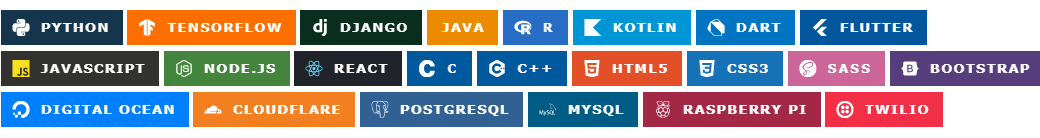
\includegraphics[width=100mm,scale=0.6]{favourite technologies 2}

% \cvevent{Product Engineer}{Google}{23 June 1999 -- 2001}{Palo Alto, CA}

% \begin{itemize}
% \item Joined the company as employe \#20 and female employee \#1
% \item Developed targeted advertisement in order to use user's search queries and show them related ads
% \end{itemize}

%\cvsection{A Day of My Life}

% Adapted from @Jake's answer from http://tex.stackexchange.com/a/82729/226
% \wheelchart{outer radius}{inner radius}{
% comma-separated list of value/text width/color/detail}
% Some ad-hoc tweaking to adjust the labels so that they don't overlap
% \wheelchart{1.5cm}{0.5cm}{%
%   10/10em/accent!30/Sleeping \& dreaming about work,
%   25/9em/accent!60/Public resolving issues with Yahoo!\ investors,
%   5/13em/accent!10/\footnotesize\\[1ex]New York \& San Francisco Ballet Jawbone board member,
%   20/15em/accent!40/Spending time with family,
%   5/8em/accent!20/\footnotesize Business development for Yahoo!\ after the Verizon acquisition,
%   30/9em/accent/Showing Yahoo!\ employees that their work has meaning,
%   5/8em/accent!20/Baking cupcakes
% }

\clearpage

% \cvsection[page2sidebar]{Publications}

\nocite{*}

% \printbibliography[heading=pubtype,title={\printinfo{\faBook}{Books}},type=book]

% \divider

% \printbibliography[heading=pubtype,title={\printinfo{\faFileTextO}{Journal Articles}}, type=article]

% \divider

% \printbibliography[heading=pubtype,title={\printinfo{\faGroup}{Conference Proceedings}},type=inproceedings]

% %% If the NEXT page doesn't start with a \cvsection but you'd
% %% still like to add a sidebar, then use this command on THIS
% %% page to add it. The optional argument lets you pull up the
% %% sidebar a bit so that it looks aligned with the top of the
% %% main column.
% % \addnextpagesidebar[-1ex]{page3sidebar}


\end{document}
